\section{Dữ liệu 3}

Bộ dữ liệu ghi lại tỷ lệ tai nạn, gồm 39 quan trắc được thực hiện trên vài đoạn đường cao tốc ở tiểu bang Minnesota vùng Trung Tây của Hoa Kỳ.

$*$ \textbf{Phương pháp chọn: Stepwise từng bước; Tiêu chuẩn chọn: BIC}.

\subsection*{Tìm hiểu dữ liệu}

Bộ dữ liệu gồm 1 biến phụ thuộc và 13 biến giải thích sau:
\begin{itemize}[label=--]
	\item $Y$ : tỷ lệ \% tai nạn trên đoạn đường khảo sát.
	\item $X1$ : chiều dài đoạn đường (dặm).
	\item $X2$ : lượng giao thông trung bình hàng ngày (nghìn xe).
	\item $X3$ : tỷ lệ \% xe tải trên tổng số.
	\item $X4$ : tốc độ giới hạn cho phép (dặm/giờ).
	\item $X5$ : chiều rộng làn đường (bước chân).
	\item $X6$ : chiều rộng làn đường khẩn cấp (bước chân).
	\item $X7$ : số làn đường thay đổi tự do trên đoạn đường cao tốc.
	\item $X8$ : số làn đường thay đổi (báo hiệu) trên đoạn đường cao tốc.
	\item $X9$ : số cửa vào đoạn đường cao tốc.
	\item $X10$ : tổng số làn đường (trên hai chiều của đường cao tốc).
	\item $X11$ : 1 nếu là tuyến đường liên thông xa lộ và cao tốc, 0 nếu ngược lại.
	\item $X12$ : 1 nếu là tuyến đường lớn của cao tốc, 0 nếu ngược lại.
	\item $X13$ : 1 nếu là tuyến đường cao tốc chính, 0 nếu ngược lại.
\end{itemize}

Một vài quan trắc đầu tiên trong bộ dữ liệu được thể hiện trong hình \ref{fig-b3:head-dataset}.
\begin{figure}[H]
	\centering
	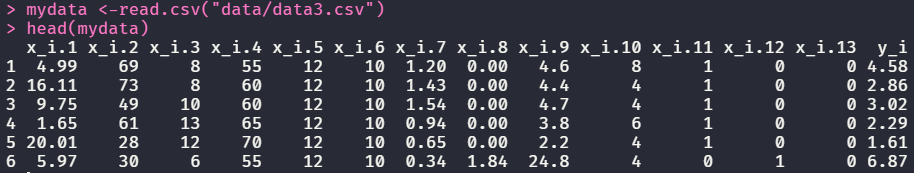
\includegraphics[width=0.8\linewidth]{images/B3/head-dataset}
	\caption{Một vài quan trắc đầu tiên}
	\label{fig-b3:head-dataset}
\end{figure}

Một số phân bố theo biến:
\begin{itemize}
	\item $X4$: Có 33 trong 39 quan trắc có tốc độ tối đa là 50, 55 và 60 (hình \ref{fig-b3:plot-x4}).
	\begin{figure}[H]
		\centering
		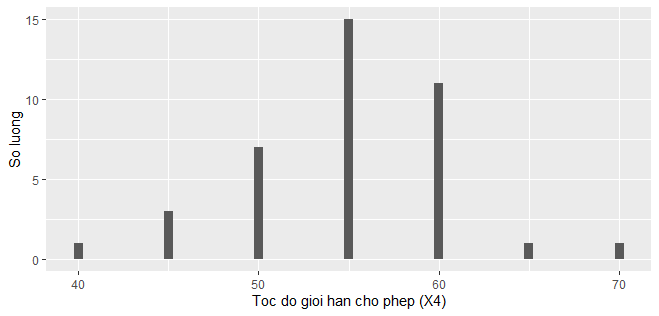
\includegraphics[width=0.7\linewidth]{images/B3/plot-x4}
		\caption{Phân bố theo tốc độ giới hạn cho phép ($X4$) (dặm/giờ)}
		\label{fig-b3:plot-x4}
	\end{figure}
	\item $X10$: Có 32 trong 39 quan trắc có tổng số làn đường là 2 hoặc 4 (hình \ref{fig-b3:plot-x10}).
		\begin{figure}[H]
			\centering
			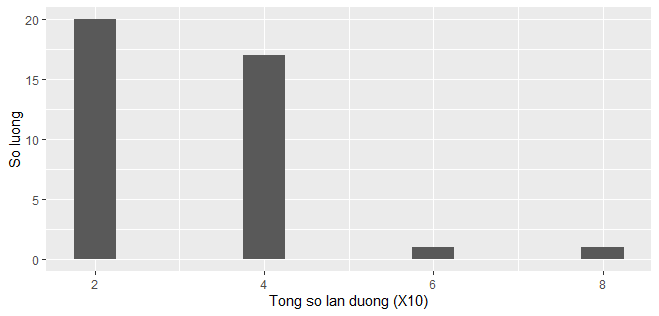
\includegraphics[width=0.7\linewidth]{images/B3/plot-x10}
			\caption{Phân bố theo tổng số làn đường ($X10$)}
			\label{fig-b3:plot-x10}
		\end{figure}
	\item $Y$: Phần lớn tỷ lệ tai nạn là $1-5\%$ (hình \ref{fig-b3:plot-y}).
		\begin{figure}[H]
			\centering
			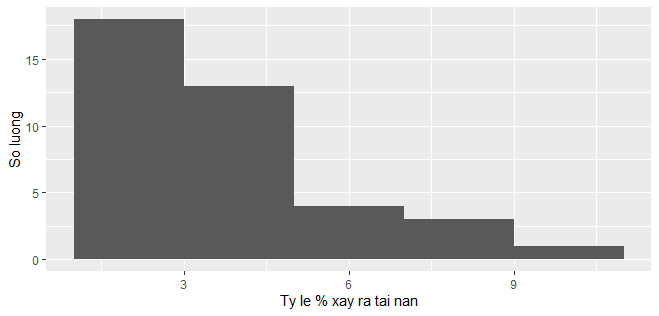
\includegraphics[width=0.7\linewidth]{images/B3/plot-y}
			\caption{Phân bố theo tỷ lệ \% tai nạn ($Y$)}
			\label{fig-b3:plot-y}
		\end{figure}
\end{itemize}

Trung bình của tổng tỷ lệ tai nạn theo các loại tuyến đường (hình \ref{fig-b3:aggregate-x11-13}) cho thấy loại tuyến đường cao tốc chính có tỷ lệ tai nạn cao nhất.
\begin{figure}[H]
	\centering
	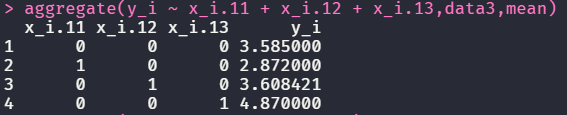
\includegraphics[width=0.7\linewidth]{images/B3/aggregate-x11-13}
	\caption{Trung bình của tổng tỷ lệ tai nạn theo các loại tuyến đường}
	\label{fig-b3:aggregate-x11-13}
\end{figure}

Trung bình của tổng tỷ lệ \% tai nạn theo các mức tốc độ giới hạn cho phép (hình \ref{fig-b3:aggregate-x4}) cho thấy giới hạn tốc độ cho phép trên đường cao tốc càng thấp thì xảy ra tai nạn càng nhiều, tỷ lệ tai nạn giảm dần khi giới hạn tốc độ cho phép tăng.
\begin{figure}[H]
	\centering
	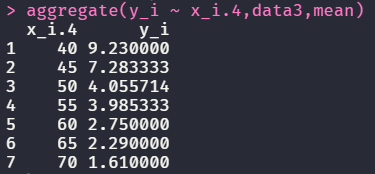
\includegraphics[width=0.45\linewidth]{images/B3/aggregate-x4}
	\caption{Trung bình của tổng tỷ lệ \% tai nạn theo các mức tốc độ giới hạn cho phép}
	\label{fig-b3:aggregate-x4}
\end{figure}

Trung bình của tổng tỷ lệ \% tai nạn theo tổng số làn đường (hình \ref{fig-b3:aggregate-x10}) cho thấy  trên đoạn đường có 8 làn đường có tỷ lệ xảy ra tai nạn cao nhất, kế đến là đoạn đường có 2 làn.
\begin{figure}[H]
	\centering
	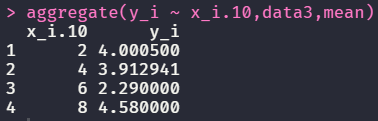
\includegraphics[width=0.45\linewidth]{images/B3/aggregate-x10}
	\caption{Trung bình của tổng tỷ lệ \% tai nạn theo tổng số làn đường}
	\label{fig-b3:aggregate-x10}
\end{figure}

Ma trận ở hình \ref{fig-b3:dataset-corr} thể hiện độ tương quan giữa các biến, cho thấy tốc độ giới hạn cho phép ($X4$) có tương quan nghịch và số cửa đoạn đường cao tốc ($X9$) có tương quan thuận đối với tỷ lệ \% tai nạn ($Y$).
\begin{figure}[H]
	\centering
	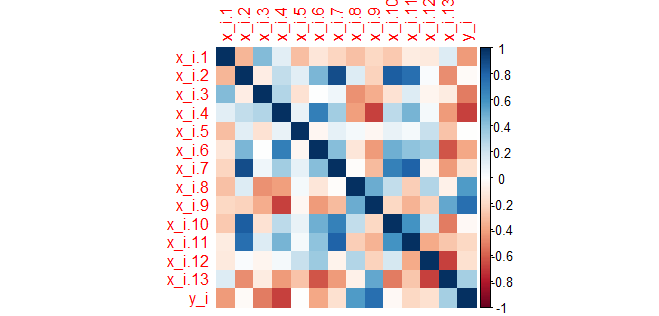
\includegraphics[width=0.85\linewidth]{images/B3/dataset-corr}
	\caption{Ma trận tương quan giữa các biến}
	\label{fig-b3:dataset-corr}
\end{figure}

\subsection*{Phân tích, chọn mô hình}

Đầu tiên, ta xét mô hình đầy đủ có dạng:
\begin{equation}\label{b3-model-full}
	\begin{split}
		Y = \beta_0 + &\beta_1X1 + \beta_2X2 + \beta_3X3 + \beta_4X4 + \beta_5X5 + \beta_6X6 + \beta_7X7\\ + &\beta_8X8 + \beta_9X9 + \beta_{10}X10 + \beta_{11}X11 + \beta_{12}X12 + \beta_{13}X13 + \epsilon
	\end{split}
\end{equation}

Mô hình hồi quy đầy đủ có các thông số ở hình \ref{fig-b3:model-full}, ta thấy được gần như tất cả 13 biến đều không có ý nghĩa thống kê. Ta tiến hành kiểm tra hiện tượng đa cộng tuyến có trong mô hình này sử dụng phương pháp tính hệ số VIF. Kết quả ở hình \ref{fig-b3:model-full-vif} cho thấy hiện tượng đa cộng tuyến xảy ra nặng nề giữa các biến, có 7/13 biến giải thích vượt ngưỡng chấp nhận được với hệ số VIF là 5 theo quy ước chung.

\begin{figure}[H]
	\centering
	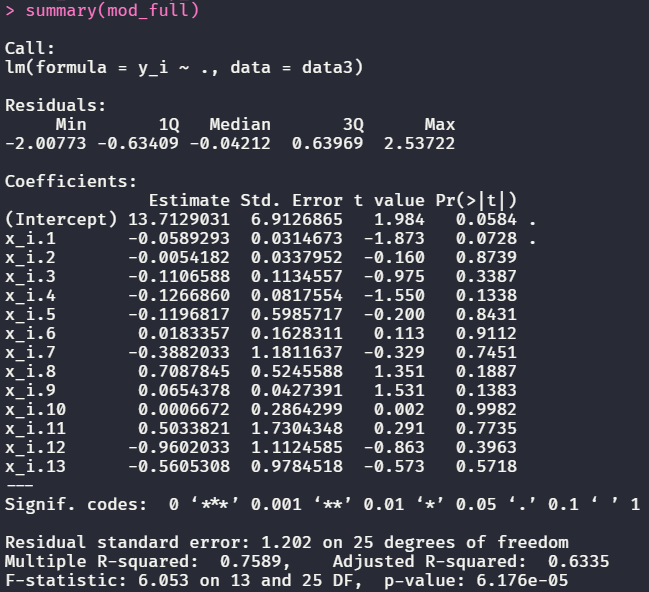
\includegraphics[width=0.65\linewidth]{images/B3/model-full}
	\caption{Mô hình hồi quy đầy đủ ban đầu}
	\label{fig-b3:model-full}
\end{figure}

\begin{figure}[H]
	\centering
	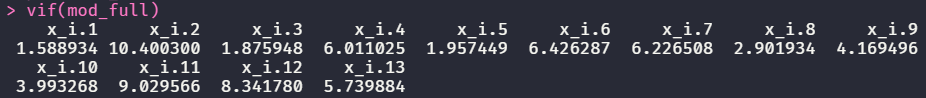
\includegraphics[width=0.8\linewidth]{images/B3/model-full-vif}
	\caption{Hiện tượng đa cộng tuyến giữa các biến trong mô hình}
	\label{fig-b3:model-full-vif}
\end{figure}

Vì số lượng biến giải thích khá ít, chỉ có 13 biến và có hiện tượng đa cộng tuyến, nên nhóm em sử dụng phương pháp hồi quy Stepwise từng bước để dễ dàng thêm bớt các biến khi chọn mô hình. Đối với tiêu chuẩn đánh giá mô hình, vì bộ dữ liệu này có cỡ mẫu nhỏ, chỉ có 39 quan trắc, nên nhóm em dùng tiêu chuẩn BIC cho cỡ mẫu $n=39$.

Dùng phần mềm R cho phương pháp Stepwise tiến lùi và tiêu chuẩn BIC, ta có kết quả ở hình \ref{fig-b3:model-bic}, mô hình lựa chọn có dạng:
\begin{equation}\label{b3-model-bic}
	Y = \beta_0 + \beta_1X1 + \beta_4X4 + \beta_9X9 + \epsilon
\end{equation}

Trong quá trình chọn mô hình, đa số các biến đã bị loại bỏ hết chỉ trừ 3 biến $X1$, $X4$, và $X9$ lần lượt giải thích cho chiều dài đoạn đường, tốc độ giới hạn cho phép và số cửa vào đoạn đường cao tốc. Mô hình \ref{b3-model-bic} có hệ số xác định $R^2 = 0.6986$ và hệ số hiệu chỉnh $R^2_{adj} = 0.6728$, các tham số ước lượng của mô hình đều có ý nghĩa thống kê. 

\begin{figure}[H]
	\centering
	\subfloat[Chọn biến]
	{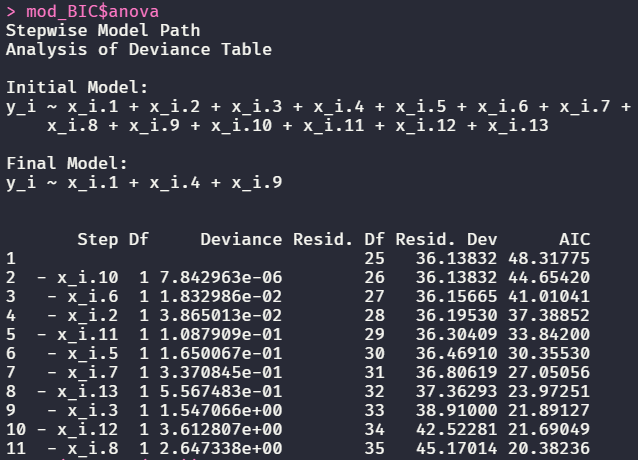
\includegraphics[width=.5\linewidth]{images/B3/model-selection-bic}}\hfill
	\subfloat[Kết quả mô hình]
	{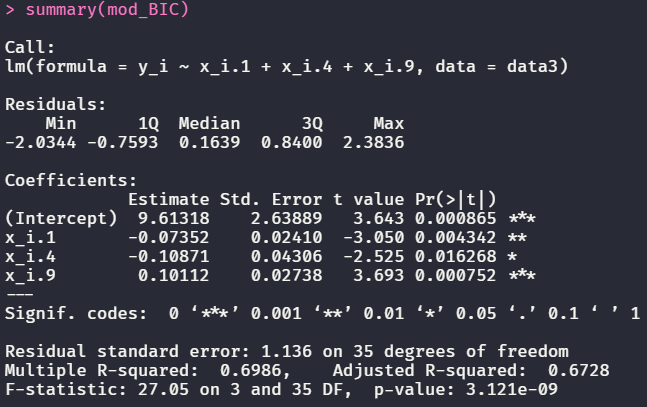
\includegraphics[width=.5\linewidth]{images/B3/model-bic}}
	\caption{Chọn mô hình với tiêu chuẩn BIC}
	\label{fig-b3:model-bic}
\end{figure}

Mô hình \ref{b3-model-bic} giải thích được 69.86\% sự biến thiên của tỷ lệ \% tai nạn được giải thích bởi 3 biến độc lập. Các hệ số của mô hình lần lượt là: $\hat{\beta_0}=9.613, \hat{\beta_1}=-0.073, \hat{\beta_4}=-0.109, \hat{\beta_9}=0.101$.

Mối tương quan giữa từng biến giải thích trong mô hình và biến phụ thuộc có quan hệ tuyến tính được biểu diễn trong hình \ref{fig-b3:model-bic-vars}. Hiện tượng đa cộng tuyến giữa các biến cũng không còn tồn tại trong mô hình được biểu diễn trong hình \ref{fig-b3:model-bic-vif}.
\begin{figure}[H]
	\centering
	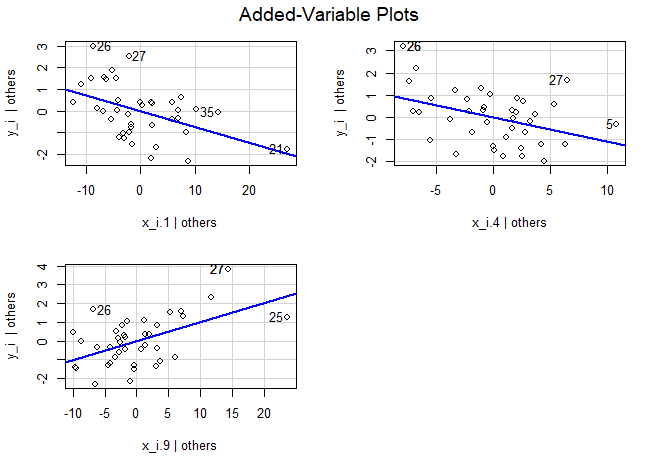
\includegraphics[width=0.65\linewidth]{images/B3/model-bic-vars}
	\caption{Mối tương quan giữa từng biến giải tích và biến phụ thuộc}
	\label{fig-b3:model-bic-vars}
\end{figure}

\begin{figure}[H]
	\centering
	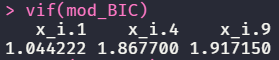
\includegraphics[width=0.35\linewidth]{images/B3/model-bic-vif}
	\caption{Hiện tượng đa cộng tuyến giữa các biến trong mô hình được chọn}
	\label{fig-b3:model-bic-vif}
\end{figure}

Tuy nhiên, biểu đồ phần dư ở hình \ref{fig-b3:model-full-plot} cho thấy mối liên quan giữa biến phụ thuộc và các biến giải thích không tuân theo hàm tuyến tính. Nhưng quan sát thấy có một số giá trị ngoại lai (\textit{outlier}) tồn tại trong dữ liệu, nhóm em sử dụng phương pháp kiểm tra là tính dao động phần dư (\textit{residuals}) và chuẩn hóa dữ liệu sao cho có trung bình 0 và phương sai 1, rồi từ đó tìm đối tượng nào có dao động phần dư chuẩn hóa cao hơn $|2|$. 
\begin{figure}[H]
	\centering
	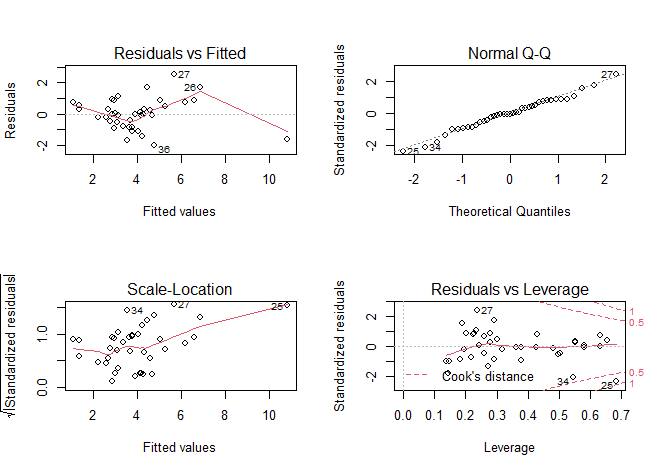
\includegraphics[width=0.65\linewidth]{images/B3/model-full-plot}
	\caption{Các biểu đồ của mô hình đầy đủ}
	\label{fig-b3:model-full-plot}
\end{figure}

Dùng phần mềm R tính toán, ta có kết quả ở hình \ref{fig-b3:dataset-outlier}, xác định được quan trắc thứ 26 và 27 là các giá trị ngoại lai.
\begin{figure}[H]
	\centering
	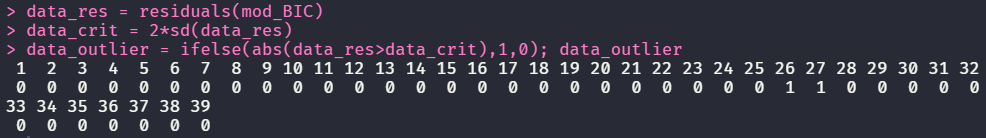
\includegraphics[width=0.7\linewidth]{images/B3/dataset-outlier}
	\caption{Kiểm tra các giá trị ngoại lai trong mô hình đầy đủ}
	\label{fig-b3:dataset-outlier}
\end{figure}

Ta thử loại bỏ các biến này và tiến hành chọn lại mô hình với phương pháp Stepwise và tiêu chuẩn BIC, ta có kết quả từ phầm mềm R ở hình \ref{fig-b3:new-models}. Mô hình lựa chọn thứ hai đã được thêm một biến $X8$ là số làn đường thay đổi (báo hiệu) trên đoạn đường cao tốc, mô hình này có dạng:
\begin{equation}\label{b3-new-model-bic}
	Y = \beta_0 + \beta_1X1 + \beta_4X4 + \beta_8X8 + \beta_9X9 + \epsilon
\end{equation}

\begin{figure}[H]
	\centering
	\subfloat[Mô hình hồi quy đầy đủ]
	{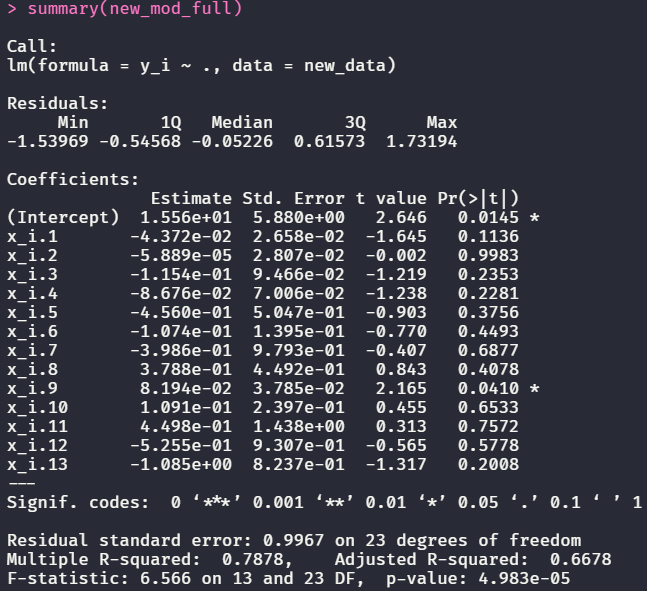
\includegraphics[width=.5\linewidth]{images/B3/new-model-full}}\hfill
	\subfloat[Mô hình lựa chọn mới với tiêu chuẩn BIC]
	{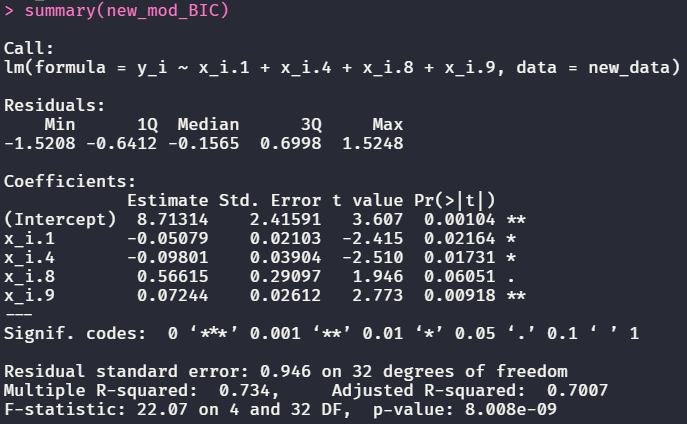
\includegraphics[width=.5\linewidth]{images/B3/new-model-bic}}
	\caption{Mô hình đầy đủ và lựa chọn sau khi loại quan trắc 26, 27}
	\label{fig-b3:new-models}
\end{figure}

Ta nhận thấy tỷ lệ phần trăm sự biến thiên giải thích được của biến phụ thuộc:
\begin{itemize}
	\item Đối với mô hình đầy đủ, có cải thiện từ 75.89\% thành 78.78\% và hệ số $R^2$ hiệu~chỉnh cũng tăng tương đối từ 0.6335 lên 0.6678. 
	\item Đối với mô hình mới \ref{b3-new-model-bic}, có cải thiện đáng kể từ 69.86\% thành 73.4\% và hệ số $R^2$ hiệu chỉnh cũng tăng tương đối từ 0.6728 lên 0.7007. 
\end{itemize}

Dù vậy, các biến trong mô hình lựa chọn mới \ref{b3-new-model-bic} lại kém có ý nghĩa thống kê hơn mô hình lựa chọn cũ. Nếu chúng ta dự trên tỷ lệ phần trăm giải thích được cho mô hình thì mô hình mới vẫn là một lựa chọn không tồi. Các biến trong mô hình vẫn đảm bảo mối quan hệ tuyến tính với biến phụ thuộc và không xảy ra hiện tượng đa cộng tuyến theo chỉ số VIF (hình \ref{fig-b3:new-model-bic-vars}, \ref{fig-b3:new-model-bic-vif}), tuy nhiên, biểu đồ phần dư cũng không thay đổi nhiều so với mô hình cũ (hình \ref{fig-b3:new-model-bic-plot}).
\begin{figure}[H]
	\centering
	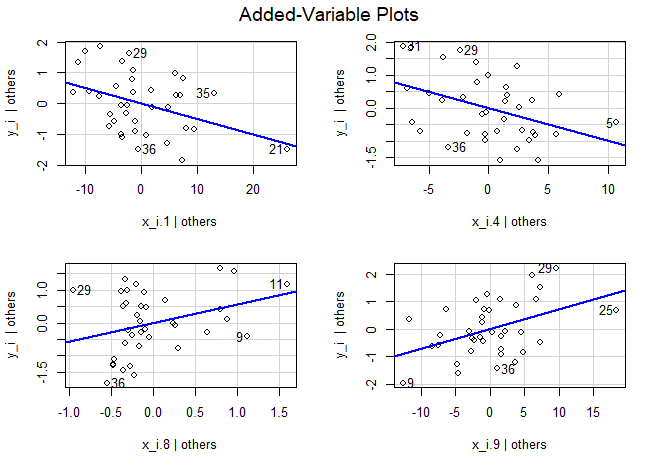
\includegraphics[width=0.7\linewidth]{images/B3/new-model-bic-vars}
	\caption{Mối tương quan giữa từng biến giải tích và biến phụ thuộc}
	\label{fig-b3:new-model-bic-vars}
\end{figure}

\begin{figure}[H]
	\centering
	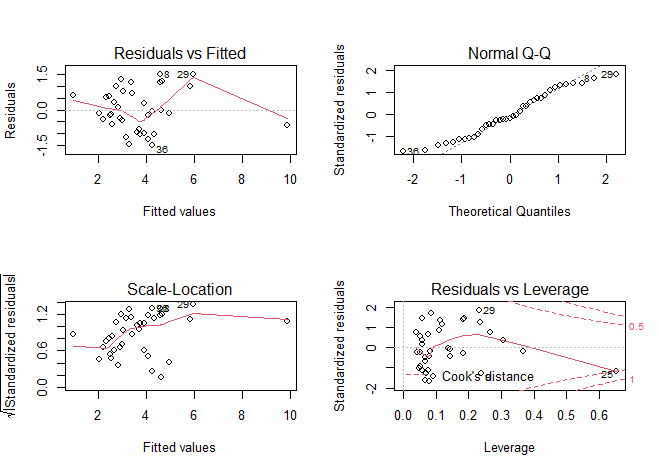
\includegraphics[width=0.7\linewidth]{images/B3/new-model-bic-plot}
	\caption{Các biểu đồ của mô hình lựa chọn mới}
	\label{fig-b3:new-model-bic-plot}
\end{figure}

\begin{figure}[H]
	\centering
	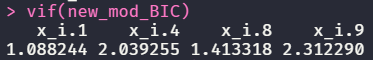
\includegraphics[width=0.45\linewidth]{images/B3/new-model-bic-vif}
	\caption{Hiện tượng đa cộng tuyến giữa các biến trong mô hình được chọn}
	\label{fig-b3:new-model-bic-vif}
\end{figure}

\subsection*{Kết luận}

Khi kiểm tra các điều kiện ý nghĩa của mô hình:
\begin{itemize}
	\item Vấn đề đa cộng tuyến trong cả hai mô hình lựa chọn đều được đảm bảo là không xảy ra.
	\item Tuy nhiên, phần dư $\epsilon$ trong cả hai mô hình đều không tuân theo phân phối chuẩn, kỳ vọng không bằng 0 và phương sai không là một hằng số.
\end{itemize}

Vậy \textbf{mô hình không có ý nghĩa}, tuy rằng mô hình lựa chọn cuối cùng đã có thể giải thích 73.4\% phương sai của biến phụ thuộc $Y$, nói cách khác, có 73.4\% phần trăm sự biến thiên của tỷ lệ tai nạn ($Y$) có thể được giải thích bởi chiều dài đoạn đường ($X1$), tốc độ giới hạn cho phép ($X4$), số làn đường thay đổi tự do trên đoạn đường cao tốc và số cửa vào đường cao tốc.

Mặt khác, dù giải pháp loại bỏ giá trị ngoại lai là cần thiết, nhưng vì dữ liệu quá ít, lý do vì sao bộ dữ liệu có những giá trị ngoại lai này vẫn chưa thể giải thích được chúng có thật sự là giá trị ngoại lai. Vì vậy, chúng ta cần nhiều dữ liệu hơn để mô hình có thể cho kết quả hồi quy tốt và chính xác hơn.